\documentclass[../main.tex]{subfiles}
\begin{document}
\section*{Word Problems}
    \begin{questions}
    \setcounter{question}{55}
    
    % Units 1 & 2
    \question[1] You are about to go base jumping and are second guessing if the cliff you are standing on is tall enough. You ask your friend to help you measure the height, so she goes down to the bottom of the cliff to help you measure the height. She starts at the base of the cliff and walks out 100 meters. You measure an angle of depression of $44^\circ$ from the horizon to her. When you base jump, you prefer to be at least 100 meters above the ground to give yourself time to safely deploy your parachute. Should you attempt this base jump? Give a mathematical reason for your decision.
    % This problem was taken directly from a past test.

        \vspace{0.5cm}
        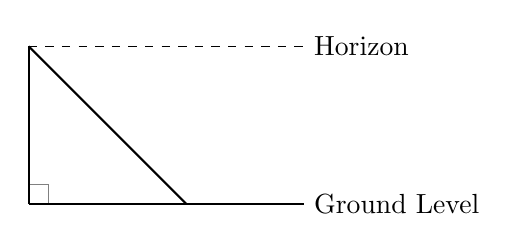
\begin{tikzpicture}[scale=.5]
        \draw [gray] (0,0) rectangle (0.5,0.5);
        \draw[black, thick] (0,0) -- (0,4);
        \draw[black, thick] (0,0) -- (7,0);
        \draw[black, thick] (0,4) -- (4,0);
        \draw[dashed]  (0,4) -- (7,4);
        \node[right] at (7,0) {Ground Level};
        \node[right] at (7,4) {Horizon};
        \end{tikzpicture} \vspace{\stretch{1}}
        
    % Unit 3
        % This problem has been copied directly from a previous test.

    \question[1] You are given an 8.5in $\times$ 11.5in piece of paper. After using it, you decide to cut out a square of the same size from each corner. After you cut out the squares, you fold the paper into an open box.
        \begin{parts}
            \part Draw a diagram for the piece of paper and for the open top box. Include variables and known values. \vspace{\stretch{2}}
    
            \part What is the interval for plausible $x$ values, where x is the side length of the square you cut out? \vspace{\stretch{2}}
            
            \part What is the equation for volume, with respect to $x$? \vspace{\stretch{2}} 
            
            \part What is the $x$ value that maximizes the volume? \vspace{\stretch{2}} 
            
            \part What is the maximum volume?
            \vspace{\stretch{2}}
            \end{parts}
    
    \newpage
  
    % Unit 4
    \question[1] How much pure acid must be added to 75 mL of a 50\% acid solution in order to produce a mixture that is 80\% acid? \vspace{\stretch{1}}
    
    \question[1] Find the dimensions of the rectangle with minimum perimeter if its area is 400 square feet. Find this least perimeter. 
    \vspace{\stretch{1}}
    
    % Unit 5
    \question[1] Given $A = Pe^{rt}$, suppose Rob invests $\$150$ at a $12\%$ interest rate compounded continuously. Find the value of his investment at the end of 6 years. 
    \vspace{\stretch{1}}
    
    \question[1] Assume Harper invests \$1200 at an 8\% interest rate compounded quarterly. 
    \newline Given $A = P(1 + \frac{r}{n})^{(nt)}$, how much money will she have in 3 years?
    \vspace{\stretch{1}}
    
    \question[1] Suppose Jim invests \$800 at an 9\% interest rate compounded quarterly. 
    \newline Given $A = P(1 + \frac{r}{n})^{(nt)}$, how much will he have \textbf{earned} in 4 years? \vspace{\stretch{1}}
    
    \question[1] Warren Buffett invested \$20,000 twice into two separate bank accounts (his total investment was \$40,000). One account pays 2\% in interest monthly and the other pays 6\% in interest annually. Given $A = P(1 + \frac{r}{n})^{(nt)}$, determine how much money, in total, he \textbf{earned} over the course of two years. \vspace{\stretch{1}}
    
    % Unit 6
    \question[1] The angle of depression from the top of a lighthouse 250ft above sea level to a sailboat is $12^\circ$. How far is the boat from the base of the lighthouse? \vspace{\stretch{2}}

    \question[1] A wire stretches from the top of a tower to the ground 40ft away from the base of the tower. The wire makes an angle of $70^\circ$ with the ground. Find the height of the tower and the length of the wire. 
    \vspace{\stretch{2}}
    
    \newpage
    
    % Unit 7
    \question[1] Two points, $A$ and $B$, are on the same side of a canyon and are 70ft apart. A hiker is located across the rim at point $C$. A surveyor determines that $\angle BAC$ is $60^\circ$ and $\angle ABC$ is $65^\circ$.
    \begin{parts}
        \part Sketch a diagram of this situation.
        \vspace{\stretch{2}}
        
        \part What is the distance between the hiker and point $A$? \vspace{\stretch{2}}
        \end{parts}
     
    \question[1] A boat leaves Miami and heads due east for 35km. At the same time, a second boat also travels from Miami for 25km. The two boats are 15.2km apart when they reach their final destination.
        \begin{parts} 
        \part Sketch a diagram of this situation. \vspace{\stretch{2}}
    
        \part What was the angle between the two boats when they left Kingston? \vspace{\stretch{2}}
        \end{parts} 
        
    % Unit 8
    \question[1] A ship is heading due north at 16mph. The current is flowing southwest at 5mph. 
        \begin{parts}
            \part Sketch a diagram of this scenario.
            \vspace{\stretch{2}}
    
            \part Find the actual bearing and speed of the ship. \vspace{\stretch{2}} \end{parts}
    
    \newpage
    \question[1] The admission fee at the Iowa state fair is \$1.50 for children and \$4.00 for adults. On a certain day, 2200 people enter the fair and \$5,050 is collected. How many children and how many adults attended? \vspace{\stretch{1}}
    
    \question[1] At a movie premiere, 351 tickets were sold. The cost for child admission was \$1.50 per ticket and the cost for adult admission was \$2.00. What was the total price of the adult tickets? \vspace{\stretch{1}} 
    
    \question[1] An exam worth 145 points contains 50 questions. Some of the questions are worth two points and some are worth five points. How many two point questions are on the test? How many five point questions are on the test? \vspace{\stretch{1}}
    \end{questions}
\end{document}